% This is LLNCS.DEM the demonstration file of
% the LaTeX macro package from Springer-Verlag
% for Lecture Notes in Computer Science,
% version 2.4 for LaTeX2e as of 16. April 2010
%
\documentclass{llncs}
%
%\usepackage{makeidx}  % allows for index generation
\usepackage{cite}
\usepackage{color}
%\usepackage{balance} % Not needed for llncs
\usepackage{times}
\usepackage{url}
\urlstyle{same} % formats footnotes
\usepackage{xcolor}
\usepackage{pgfplots}
\usepackage{soul} % highlighting
%\usepackage{multirow}
\usetikzlibrary{patterns} %% Used for bar charts
\usepackage{float} %% Used for side by side minipages


\usepackage{amssymb}% Checkmark

\newcommand{\todo}[1]{\textcolor{cyan}{\textbf{[#1]}}}
\newcommand{\dan}[1]{\textcolor{blue}{{\it [Dan says: #1]}}}
\newcommand{\andy}[1]{\textcolor{blue}{{\it [Andy says: #1]}}}
\newcommand{\sam}[1]{\textcolor{blue}{{\it [Sam says: #1]}}}

% Define flow chart styles
\tikzstyle{decision} = [diamond, draw, fill=blue!20,
    text width=15em, text badly centered, node distance=3cm, inner sep=0pt]
\tikzstyle{block} = [rectangle, draw, fill=blue!20,
    text width=15em, text centered, rounded corners, minimum height=4em]
\tikzstyle{line} = [draw, -latex']

\usetikzlibrary{shapes,arrows, positioning} % Needed for analysis diagram


\newif\ifisnopii
\isnopiitrue % change to true/false to remove personally identifiable information (pii)
%\isnopiifalse % change to true/false to remove personally identifiable information (pii)





%
\begin{document}
%
\frontmatter          % for the preliminaries
%
\pagestyle{headings}  % switches on printing of running heads
%

\mainmatter              % start of the contributions
%
\title{Mistakes and Malware: A Large Scale Analysis of Benign and Malicious Android Apps}
%
\titlerunning{Title-21}  % abbreviated title (for running head)
%                                     also used for the TOC unless
%                                     \toctitle is used
%
%\author{Ivar Ekeland\inst{1} \and Roger Temam\inst{2} Jeffrey Dean \and David Grove \and Craig Chambers \and Kim~B.~Bruce \and Elsa Bertino}

%\author{Ivar Ekeland\inst{1} \and Roger Temam\inst{2} Jeffrey Dean \and David Grove \and Craig Chambers \and Kim~B.~Bruce \and Elsa Bertino}

\author{Daniel E. Krutz, Andrew Meneely, Samuel A. Malachowsky, Casey Klimkowsky, Shannon Trudeau, and Adam Blaine}

%
\authorrunning{Ivar Ekeland et al.} % abbreviated author list (for running head)
\institute{Rochester Institute of Technology, Rochester, NY, USA,\\
\email{\{dxkvse, axmvse, samvse, cek3403, smt9020, amb8805\}@rit.edu}
}

\maketitle              % typeset the title of the contribution

\begin{abstract}

Android applications (apps) are not immune to the problems which also plague conventional software including security vulnerabilities, quality defects, permission misuse, and numerous other issues. Many developers even intentionally create vulnerable or malicious apps (malware) for often highly lucrative purposes. We need to better understand current trends in app quality and security order to create higher quality software, and more effectively battle malware. In order to gather this critical information, we collected and reverse engineered 70,785 Android apps from the Google Play store, along with 1,420 malicious apps from other sources. Each app was analyzed using several static analysis tools to record a variety of information about each of them including requested permissions, size (LOC), possible defects and permission misuse. Our findings conclude that: 1) app categories substantially differ in terms of permissions misuse; 2) that there is no significant correlation between an app's quality and security; 3) that malware typically requests more permissions and suffers in several quality related metrics in comparison to benign apps; 4) that malware and benign apps are annually growing both in terms of LOC and requested permissions. We also present an easy to use, robust website and dataset for others to use in their own research.


% These are not in the other papers
%\keywords{Android, Malware, Static Analysis}
\end{abstract}
%



\section{Introduction}

Android is the world's most popular mobile operating system with over 1.8 million apps available from Google Play alone~\cite{statistica_url}. In order to create better apps, we need to better understand the current trends in development, and what some of the most profound issues from a security and quality perspective are. A few areas which should be examined include permissions misuse, security vulnerabilities, defects, and adherence to coding standards. In recent academic studies, static analysis tools have been used as one method of measuring the quality and security of mobile software~\cite{Felt:2011:APD:2046707.2046779,Vidas11curbingandroid,Lee_2013, krutz2015FDroid}. \emph{An empirical analysis of a large body of malicious and benign Android applications over time can therefore provide insights into these apps, and their trends.}

%Unfortunately, many apps are created with a sinister intent. Malware is a constant concern as recent studies have shown that nearly 20\% of Android apps are malware~\cite{tynan_dan_report:_2015}. In order to better detect and defend against malware, we need to understand more about it. Knowing how it is created, evolves, and its characteristics are all valuable pieces of information in the battle against malware.

The goal of this work is to better understand benign and malicious Android apps through the use of static analysis. We collected and reverse engineered 70,785  Android applications (APK files) in 41 different categories from Google Play, along with 1,420 malware samples from the Contagio Mobile Mini Dump~\cite{contagio_url} and the Malware Genome Project~\cite{Zhou:2012:DAM:2310656.2310710}. Each app was analyzed using five static analysis tools: Stowaway~\cite{Felt:2011:APD:2046707.2046779}, Androrisk\footnote{\url{https://github.com/androguard/androguard}}, CheckStyle\footnote{\url{http://checkstyle.sourceforge.net/}}, Jlint\footnote{\url{http://jlint.sourceforge.net/}}, and APKParser\footnote{\url{https://github.com/joakime/android-apk-parser}}. We examined application size, rate of potential defects, adherence to coding standards, rate of permissions misuse, and security risk level. We have also created a publicly available dataset and robust website which may be used by researchers, developers, students, and general Android users to better understand these apps. Our work is guided by the following research questions:

%We found that `Tools' apps suffer from the highest rate of coding standards defects per line of code (LOC), while `Communication' apps have the highest rate of over-permission.

%%%
\noindent
\textbf{RQ1:}~\emph{How do app categories compare in terms of several security metrics?} We found that app categories significantly differ in terms of size, and other permissions based security metrics. Some of the evaluated areas include number of requested permissions, and permission gap.

% (`Books \& Reference: 5.4 '-`Communication: 14.6), and over-permissions (`Puzzle': 2 - `Communication':5).

%%%
\noindent
\textbf{RQ2:}~\emph{What are the most pervasive over-permissions?} We found that some of the most common over-permissions in Google Play apps include \texttt{GET\_ACCOUNTS}, \texttt{CALL\_PHONE}, \texttt{READ\_EXTERNAL\_STORAGE}, and \texttt{ACCESS\_WIFI\_STATE}.
%%%

\noindent
\textbf{RQ3:}~\emph{Is there a correlation between quality \& security?} We found only a weak association between the quality and security of apps in the several evaluated comparisons.

%%%
\noindent
\textbf{RQ4:}~\emph{How do benign \& malicious Android apps compare in terms of several security based metrics?} Our results indicate that malicious apps typically contain more over-permissions, and total requested permissions, while Google Play apps have a larger rate of under-permissions and Androrisk score.

%%%
\noindent
\textbf{RQ5:}~\emph{How are apps changing over time?} We found that both malicious and benign apps are annually growing in terms of both LOC and requested permissions.

The rest of the paper is organized as follows: Section~\ref{sec: relatedwork} discusses related works, while Section~\ref{sec: androidPermissions} describes the Android permissions model. Section~\ref{sec: csa} provides details of how we collected the apps and conducted our static analysis on them. Section~\ref{sec: evaluation} discusses the results of our research questions and analyzes our findings. Section~\ref{sec:dataset} presents information regarding our public dataset. Section~\ref{sec:limitations} discusses limitations of our research and future work to be conducted, while Section~\ref{sec: conclusion} concludes our study.
%\dan{make sure this is up to date}

\section{Related Work}
\label{sec: relatedwork}

There have been several studies which analyzed mobile apps on a large scale. Sarma~\emph{et al.} evaluated several large data sets, including one with 158,062 Android apps in order to gauge the risk of installing the app, with some of the results broken down by category. However, this work did not analyze the apps using the range of static analysis tools which we used. Viennot~\emph{et al.} developed a tool called `PlayDrone' which they used to examine the source code of over 1,100,000 free Android apps. While the authors studied a very large number of apps, they largely only used existing information which could be gathered from Google Play and only examined features such as library usage and duplicated code. They did not study areas such as security risk levels, quality attributes, or the permission gap, which were a part of our analysis. Felt~\emph{et al.} described some common developer errors found using their tool Stowaway, including confusing permission names, the use of depreciated permissions, and errors due to copying and pasting existing code~\cite{Felt:2011:APD:2046707.2046779}. In another work, Felt~\emph{et al.} very briefly described some inclinations they had for why developers gave too many permissions to applications, but this was largely based on assumptions and not necessarily data~\cite{Felt:2011:EAP:2002168.2002175}.

%%% Talk about how these works also examined the permissions gap ?
%%% What we did was much newer than what they worked on. Their study is several years old?


Grace et al.\cite{Grace:2012:UEA:2185448.2185464} conducted work on permissions probing, which is when a 3rd party component attempts to use a permission in the hope that the attached app has requested it from the user. If the attached app has requested a permission, then the component will also have access to that permission as well. This is often done to collect, and transmit potentially sensitive information which should not be normally available to the 3rd party component. They found that more than half of all ad libraries try to probe for open permissions. This could often be the cause of an under-permission in an app since the ad library will try to use a permission which the developer did not request.

Stevens~\emph{et al.}\cite{6624000} analyzed 10,000 free Android apps and found a strong sub-linear relationship between the popularity of a permission and the frequency of its misuse. They found that developers were more likely to misuse a permission when they did not understand it, and that the popularity of a permission is strongly associated with its misuse. A powerful method of avoiding permission misuse is through developer education and community support. Krutz~\emph{et al.}\cite{krutz2015FDroid} created a public dataset of over 1,100 Android apps from the F-Droid\footnote{https://f-droid.org/} repository. This research analyzed a much smaller number of apps than our study and focused more on the life cycle of the apps and how each iteration of the app evolved with every version control commit.

%% Take out of space is an issue
There are several other websites which gather metrics about Android apps. One of the most popular is AppAnnie\footnote{\url{https://www.appannie.com}} which collects Android apps and performs several types of analysis on each of them including downloads of the app over time and advertising analytics. However, no known services perform the same types of static analysis and comparisons on apps that we do.

A substantial amount of research has been conducted on Android malware ranging from various detection techniques~\cite{6799722, Feng:2014:ASD:2635868.2635869, Rastogi:2013:DEA:2484313.2484355} to reconstructing malware behavior~\cite{reina2013system}. Zhou et al.\cite{zhou2012dissecting} analyzed a large number of malware samples and characterized them in several areas including installation techniques, activation methods, and nature of malicious payloads. Unfortunately, the newest of these malware samples was only from 2011, and did not compare malicious and benign apps against one another, or use the range of static analysis tools as in our work.

\section{Android Permissions}
\label{sec: androidPermissions}

Android apps operate under a permission-based system where an app requires specific permissions to carry out specific functionality. In Android versions \textless 6.0, the user is asked to accept or reject the requested permissions when installing the app. Beginning with Android 6.0, users may be asked for these permissions during runtime. Unfortunately, developers often request more permissions than they actually need, as there is no built in verification system to ensure that they are only requesting the permissions their application actually uses~\cite{Felt:2011:APD:2046707.2046779}. In this study, we use the term \emph{over-permission} to describe a permission setting that grants more than what a developer needs for the task. Likewise, an \emph{under-permission} is a setting for which the app could fail because it was not given the proper permissions. If not properly handled, an application, could throw a~\emph{SecurityException} when it attempts to perform an operation which it does not have permission to conduct.

Over-permissions are considered security risks since they do not adhere to the~\emph{principle of least privilege} and unnecessarily increase an app's attack surface. Under-permissions are considered quality risks, with a possible indication of permission probing. The primary difference between requested permissions and over-permissions is that requested permissions are merely those that the app asks to use, and does not take into consideration if the app actually needs them or not. While largely a quality concern, under-permissions can represent a possible security concern as well. One example of this is when permissions are, unknowingly to the developer, misused in a variety of ways by 3rd party libraries or even by associated ad networks which may collect and transmit potentially sensitive user data~\cite{Grace:2012:UEA:2185448.2185464}.

%% Taken out for space reasons
%The~\emph{principle of least privilege} is the concept of granting of the least amount of privileges to an application that it needs to properly function~\cite{saltzer1975protection}. Granting extra privileges creates unnecessary security vulnerabilities by allowing malware to abuse these unused permissions, even in benign apps~\cite{6624000}. These extra privileges also increase the app's attack surface~\cite{Davi:2010:PEA:1949317.1949356, Bartel:2012:ASP:2351676.2351722}. Previous research has found that Android developers often mistakenly add unnecessary privileges in a counterproductive and futile attempt to make the app work properly, or due to confusion over the permission name they add it incorrectly believing its functionality is necessary for their app~\cite{Felt:2011:APD:2046707.2046779}. While largely a quality concern, under-permissions can represent a possible security concern as well. One example of this is when permissions are, unknowingly to the developer, misused in a variety of ways by 3rd party libraries or even by associated ad networks which may collect and transmit potentially sensitive user data~\cite{Grace:2012:UEA:2185448.2185464,7371575}.



\section{Collection \& Static Analysis}
\label{sec: csa}

We analyzed apps collected from Google Play and several malware sources using a variety of different tools. The results of this analysis have been stored in a publicly accessible database located on our project website\footnote{\ifisnopii http://darwin.rit.edu \else http://xxx.hiddenToKeepAnonymous.edu \fi}. An overview of the collection and analysis process is shown in Figure~\ref{fig:analysisprocess}.

\begin{figure}[h]

\begin{center}

% Define block styles
\tikzstyle{line} = [draw, -latex']

%\tikzstyle{cloud} = [draw, ellipse,fill=white!20, node distance=1.5cm, minimum height=2em]
\tikzstyle{cloud} = [draw=none, ellipse,fill=white!20, node distance=1.5cm, minimum height=2em]

\tikzstyle{block} = [rectangle, draw, fill=white!20, text width=5em, text centered, rounded corners, minimum height=4em]
\tikzstyle{c} = [draw, cylinder, shape border rotate=90, aspect=0.75, minimum height=70, minimum width=30]

\scalebox{.9}{
\begin{tikzpicture}[node distance = 1.5cm, auto]

    % Place nodes
     \node [cloud] (init) {APK Collection};
     \node [block, below of=init] (ApkFiles) {ApkFiles};
     \node [cloud, below of=ApkFiles] (Decompile) {Decompile};
     \node [block, below of=Decompile] (DecompiledFiles) {Decompiled Files};
     \node [cloud, below of=DecompiledFiles] (JavaAnalysis) {Java Analysis};
    % \node [cloud, right of=ApkFiles] (apkanalysis) {Stowaway Androrisk};
    % \node [c, right of=DecompiledFiles] (SqliteDB) {SqliteDB};
     \node[c] (SqliteDB) [below right=-1.0cm and 2.4cm of DecompiledFiles]{SQLiteDB};

    \node[cloud] (apkanalysis) [below right=-0.9cm and 2.0cm of ApkFiles]
       {APK Analysis};

    % Draw edges
    \path [line] (init) -- (ApkFiles);
    \path [line] (ApkFiles) -- (Decompile);
    \path [line] (Decompile) -- (DecompiledFiles);
    \path [line] (DecompiledFiles) -- (JavaAnalysis);
    \path [line] (ApkFiles) -- (apkanalysis);
    \path [line] (apkanalysis) -- (SqliteDB);
    \path [line] (JavaAnalysis) -- (SqliteDB);
    \path [line] (Decompile) -- (SqliteDB);

\end{tikzpicture}
} % scale
\caption{APK Analysis Process}
\label{fig:analysisprocess}
\end{center}
\end{figure}






%Our methodology is as follows:
%
%\begin{enumerate}
%    \setlength{\itemsep}{0pt} %Cut down on spacing for the different items in the list
%    \setlength{\parskip}{0pt} %Cut down on spacing for the different items in the list
%    \setlength{\parsep}{0pt}  %Cut down on spacing for the different items in the list
%
%  \item Collect APK files.
%  \item Reverse-engineer binaries.
%  \item Execute static analysis tools.
%  \item Complete evaluation process.
%\end{enumerate}



%%% Removed due to splace
%%There were several significant challenges which had to be overcome in our collection and analysis process. A goal for our project was to run our collection tool for over a year to ensure that we were collecting a diverse set of apps, along with numerous versions of many of the apps. During this time, there were many small alterations that Google made which affected our collection process which created a need for our system to be regularly modified to continue functioning properly. Accuracy for our process was a paramount concern since problems with even a very small percentage the apps at any stage in the collection or reverse engineering process could have had devastating results on the accuracy of our work. In order to ensure the accuracy of our results, we relied upon unit testing, manual verification, and frequent test runs. The optimization and testing phases took up the vast majority of development time for the project.  We also made slight modifications to the existing version of Stowaway to accommodate our process and current Android applications with updated permissions.

%%% Add back in if we can think of other challenges which had to be overcome
%There were several significant challenges which had to be overcome in our collection and analysis process. We ran our collection mechanism for over a year, and during this time it needed to be regularly updated due to alterations with Google Play, which impacted this collection process.



%A goal for our project was to run our collection tool for over a year to ensure that we were collecting a diverse set of apps, along with numerous versions of many of the apps. During this time, there were many small alterations that Google made which affected our collection process which created a need for our system to be regularly modified to continue functioning properly.



%Accuracy for our process was a paramount concern since problems with even a very small percentage the apps at any stage in the collection or reverse engineering process could have had devastating results on the accuracy of our work. In order to ensure the accuracy of our results, we relied upon unit testing, manual verification, and frequent test runs. The optimization and testing phases took up the vast majority of development time for the project.  We also made slight modifications to the existing version of Stowaway to accommodate our process and current Android applications with updated permissions.



%Reverse engineering and analyzing each app was nonalso a time consuming process.

%%% Taken out for space reasons
%%Our goal was to examine a large number of apps using a diverse set of high quality and accurate tools. While there are numerous static analysis tools for analyzing software, we were limited in using those which were already demonstrated to be effective in previous research, but importantly also took less time to analyze the apps. For instance, we selected Jlint over FindBugs since it was able to analyze the applications much faster, while still providing accurate results~\cite{rutar2004comparison}. Many of the apps took 5-10 minutes to reverse engineer and analyze, so we were forced to pay heavy attention to the efficiency of the reverse engineering and analysis process which included optimizations to process and thread management.

%\vspace{-8mm}

\label{sec: collection}
\subsection{Step 1: Collect APK files}

Android APK files were pulled from Google Play with a custom-built collector, which uses~\emph{Scrapy}\footnote{http://scrapy.org} as a foundation. To limit the impact of seldom-downloaded applications, we divided of our results into two groups: applications with at least 10,000 downloads, and those with less than 10,000 downloads. Of the 70,785 apps downloaded, 31,234 had at least 10,000 downloads. The creation date of the collected apps ranged from 2011, to late 2015. We assume that these apps from Google Play are not malicious, and will often refer to them as benign apps when comparing them with malware. We only used free apps in our analysis. Malware was collected  from two well known sources, the Contagio Mobile Mini Dump~\cite{contagio_url} and the Malware Genome Project~\cite{Zhou:2012:DAM:2310656.2310710}. The Contagio Mobile Mini Dump has been collecting malware affecting many platforms, including Android, for several years. We used a total of 1,420 malware examples from 49 malware families in our analysis.




%\subsection{Step 2: Reverse-engineer binaries}
%\label{sec: decompliation}
%Jlint and Checkstyle required the downloaded APK files to be decompiled to .java files, so using dex2jar\footnote{\url{https://code.google.com/p/dex2jar/}} and jd-cmd\footnote{\url{https://github.com/kwart/jd-cmd}}, we followed a reverse engineering process that has already demonstrated itself to be effective in similar research~\cite{Lee_2013,6687155}. We also recorded the number of extracted class and java files. The de-compilation process is shown in Figure~\ref{fig:extractionprocess}.
%
%% ~\cite{Lee_2013} %% This diagram is largely copied from here
%% Define block styles
%\tikzstyle{line} = [draw, -latex']
%\tikzstyle{cloud} = [draw, ellipse,fill=white!20, node distance=2.2cm,
%    minimum height=2em]
%
%	\begin{figure}[h]
%	\begin{center}
%
%\begin{tikzpicture}[node distance = 2cm, auto]
%    % Place nodes
%     \node [cloud] (init) {.apk};
%     \node [cloud, right of=init] (dex) {.dex};
%     \node [cloud, right of=dex] (jar) {.jar};
%     \node [cloud, right of=jar] (java) {.java};
%
%     \path [line] (init) -- node {unzip}(dex);
%     \path [line] (dex) -- node {dex2jar}(jar);
%     \path [line] (jar) -- node {jd-cmd}(java);
%
%\end{tikzpicture}
%\caption{APK Extraction Process}
%\label{fig:extractionprocess}
%\end{center}
%\end{figure}
%
%While no reverse engineering process can ever be considered perfect, our utilized technique has been demonstrated to be highly effective in previous research~\cite{apvrille2012android,chawla2014transfiguring, krutz2015FDroid, Lee_2013}. We also checked the accuracy of this reverse engineering process by manually analyzing at least 10 .java files from over 50 reverse engineered Android apps in our study. Since we used an already established reverse engineering process, there were few unforeseen hurdles in our collection or reverse engineering process.
%%%% Make it known that this is not a new process, and therefore is more likely to be accurate


\subsection{Step 2. Execute static analysis tools}
\label{sec: analysis}

After reverse engineering the apps using a process established in previous works~\cite{Lee_2013,6687155}, the next phase was to analyze them for a variety of security and quality metrics. In addition to using the tools below, we also recorded other metrics about each application including total lines of code, number of Java files, application version, target SDK, and minimum SDK.

%The next phase was to analyze the extracted source code for a variety of metrics, including potential security risks, permissions issues, potential defects, and misuse of coding standards. We used the following tools for our analysis: %We also collected information about software clones, which are functionally equivalent portions of an application that may differ syntactically. A sign of poorly written software, clones may be detrimental to an application in a variety of ways, including increased maintenance costs and inconsistent bug fixes~\cite{Roy:2009:CEC:1530898.1531101}.

\textbf{Stowaway:} Reports the under-permissions and over-permissions of an application. Similar to previous work~\cite{6624000}, we made slight modifications to Stowaway to accommodate our process and stay current with updated Android permissions.

\textbf{Androrisk:} Determines the security risk level of an app by evaluating several criteria. The first is the presence of permissions which are deemed to be more dangerous. These include the ability to access the internet, manipulate SMS messages, or the rights to make a payment. The second is the presence of more dangerous sets of functionality in the app including a shared library, use of cryptographic functions, and the presence of the reflection API.


\textbf{CheckStyle:} Measures how well developers adhere to coding standards such as annotation usage, size violations, and empty block checks. We recorded the total number of violations of these standards. Default application settings for Android were used in our analysis. While adherence to coding standards may seem to be an overly fastidious thing to measure, compliance to coding standards in software development can enhance team communication, reduce program errors and improve code quality~\cite{Li:2005:ETC:1095714.1095770, li2006using}.

\textbf{Jlint:} Discovers bugs, inconsistencies, and synchronization problems by conducting a data flow analysis and building lock graphs. We recorded the total number of discovered possible defects. This tool was selected over FindBugs since it was able to analyze the applications much faster, while still providing accurate results~\cite{rutar2004comparison}.

\textbf{APKParser:} Reads various information from Android APK files including the version, intents, and requested permissions.



%Stowaway and Androrisk were able to analyze the raw APK files, while CheckStyle, Jlint, and Nicad required the APK files to be decompiled. All results were recorded in an SQLite database, which is publicly available on the project website.


\section{Evaluation}
\label{sec: evaluation}

In the following sections, we describe our findings and answer our research questions.

\subsection{RQ1: How do app categories compare in terms of several security metrics?}

Android apps are separated into different groups known as categories, some of which include `Communication', `Education', `Lifestyle', and `Tools'. These different app groups all have different focuses, likely different target audiences, and very often different developers. We sought to better understand how apps from different categories compare in terms of several metrics including use of permissions, rate of permissions misuse, and app size. Table \ref{Table:topGroups} shows the top 10 collected categories, and an aggregate of all collected apps from Google Play (not just from the top categories) along with malicious apps.

%% Categories closely align (but do not perfectly match) the categories on http://www.appbrain.com/stats/android-market-app-categories

\begin{table*}[]
%% I removed JLINT coding standards from this table since the results were not that profound.
\begin{center}
\caption{Comparison of App Groups}
\label{Table:topGroups}
 \begin{tabular}{ | l | c | c | c | c | c |  c |} \hline

%% With No CS issues
  \bfseries Group & \bfseries ~~~~ LOC ~~~~  & \bfseries Over-Permissions & \bfseries Under-Permissions & \bfseries Requested Permissions \\ \hline


 	\bfseries Arcade &	152,563	  &	2.3 &	3.8 &	6.6 \\ \hline
 	\bfseries Books \& Reference &	123,600	  &	2.6 &	2.7 &	5.4 \\ \hline
	\bfseries Casual &	150,396  &	2.2 &	4 &	6.5 \\ \hline
 	\bfseries Communication & 	166,083  &	5.2 &	3.6 &	14.6 \\ \hline
	\bfseries Education &	131,615  &	2.2 &	3.3 &	5.8 \\ \hline
 	\bfseries Entertainment &	138,229  &	2.6 &	2.8 &	6.3 \\ \hline
 	\bfseries Lifestyle &	166,114  &	2.9 &	3 &	8.2 \\ \hline
 	\bfseries Music \& Audio &	146,211	  &	2.5 &	2.7 &	6.7 \\ \hline
  	\bfseries Personalization &	113,539	   &	3.8 &	2.5 &	8.3 \\ \hline
 	\bfseries Puzzle &	142,998  &	2 &	3.8 & 	5.6 \\ \hline
	\bfseries Tools	 & 106,131  &	4.1 &	2.9 &	8.4 \\ \hline \hline

	\bfseries Avg Google Play	 & 158,689  & 3.0 &	3.3 &	7.8 \\ \hline
	\bfseries Malware	 & 32,373  & 6 &	1.9 &	 12.4 \\ \hline


%%% With CS issues
%  \bfseries Group & \bfseries LOC & \bfseries CS Mistakes/LOC & \bfseries O-Privs & \bfseries U-Privs & \bfseries Requested Privs \\ \hline
%
%
% 	\bfseries Arcade &	152,563	 &	.01048 &	2.3 &	3.8 &	6.6 \\ \hline
% 	\bfseries Books \& Reference &	123,600	 &	.00675 &	2.6 &	2.7 &	5.4 \\ \hline
%	\bfseries Casual &	150,396 &		.0103~~ &	2.2 &	4 &	6.5 \\ \hline
% 	\bfseries Communication & 	166,083  &	.06824 &	5.2 &	3.6 &	14.6 \\ \hline
%	\bfseries Education &	131,615 &	.0234~~ &	2.2 &	3.3 &	5.8 \\ \hline
% 	\bfseries Entertainment &	138,229 &	.01367 &	2.6 &	2.8 &	6.3 \\ \hline
% 	\bfseries Lifestyle &	166,114 & 	.02639 &	2.9 &	3 &	8.2 \\ \hline
% 	\bfseries Music \& Audio &	146,211	 &	.00985 &	2.5 &	2.7 &	6.7 \\ \hline
%  	\bfseries Personalization &	113,539	  & 	.06075 &	3.8 &	2.5 &	8.3 \\ \hline
% 	\bfseries Puzzle &	142,998 & 	.01025 &	2 &	3.8 & 	5.6 \\ \hline
%	\bfseries Tools	 & 106,131 &	.07202 &	4.1 &	2.9 &	8.4 \\ \hline \hline
	
	%%% Version with JLINT
%	\bfseries Arcade &	152,563	& .0027 &	.01048 &	2.3 &	3.8 &	6.6 \\ \hline
% 	\bfseries Books \& Reference &	123,600	& .0025 &	.00675 &	2.6 &	2.7 &	5.4 \\ \hline
%	\bfseries Casual &	150,396 &	.0026 &	.0103~~ &	2.2 &	4 &	6.5 \\ \hline
% 	\bfseries Communication & 	166,083 &	.0029 &	.06824 &	5.2 &	3.6 &	14.6 \\ \hline
%	\bfseries Education &	131,615 &	.0023 &	.0234~~ &	2.2 &	3.3 &	5.8 \\ \hline
% 	\bfseries Entertainment &	138,229 &	.0024 &	.01367 &	2.6 &	2.8 &	6.3 \\ \hline
% 	\bfseries Lifestyle &	166,114 & .0023 &	.02639 &	2.9 &	3 &	8.2 \\ \hline
% 	\bfseries Music \& Audio &	146,211	 & .0025 &	.00985 &	2.5 &	2.7 &	6.7 \\ \hline
%  	\bfseries Personalization &	113,539	 & .0024 & 	.06075 &	3.8 &	2.5 &	8.3 \\ \hline
% 	\bfseries Puzzle &	142,998 & .0025 &	.01025 &	2 &	3.8 & 	5.6 \\ \hline
%	\bfseries Tools	 & 106,131 &	.0025 &	.07202 &	4.1 &	2.9 &	8.4 \\ \hline
	
%	\bfseries Avg Google Play	 & 158,689 & .03065 & 3.0 &	3.3 &	7.8 \\ \hline
%	\bfseries Malware	 & 32,373 & .06867 & 6 &	1.9 &	 12.4 \\ \hline
	
	
  \end{tabular}
  \end{center}
\end{table*}



%% I took out Jlint issues since these value were not all that surprising
%%We next analyzed the rate of discovered defects in each app by dividing the number errors detect by Jlint by the app's LOC. Surprisingly, we found that there wasn't a significant difference in the number of discovered defects which ranged from .0023/LOC-.0029/LOC. There are several possible explanations for these similar values. One is that since a large portion of

We found a large variation in the rate of over-permissions for each category with `Casual' and `Education' apps having the fewest with 2.2 per app and `Communication' having the largest with 5.2 for each app. `Personalization' apps had the fewest number of under-permissions (2.5), while `Casual' apps had the highest rate with 4 per app. The `Books \& Reference' category requested the fewest permissions per app, while `Communication' apps requested the most permissions with an average of 14.6. `Lifestyle' apps were narrowly the largest with an average 166,114 LOC per app, while `Tools' apps were the smallest with 106,131 LOC.

\noindent
\textbf{Analysis:} These findings are important for a variety of reasons. The results show a wide disparity among the various categories in terms of app size and security concerns. Developers may use this information to devote more resources to specific categories in the identified permissions based issues, while for researchers it demonstrates the wide disparity in terms of size, requested permissions and the permission gap between various categories. Over-permissions are a possible security vulnerability, so app categories with more over-permissions should be given more focus from security researchers from both the perspective of why they occur, to what their negative implications may be for these categories. With the introduction of Android 6.0, future work should be done to examine the rate of change in over-permissions in the different categories with this new permissions model. Also, since over-permissions are often caused by lack of developer understanding with the abused permissions~\cite{6624000}, these categories with the most over-permissions require the most developer education.

%Due to the significant security differences between several of the categories, further work should be conducted to determine why certain categories are more successful from a security perspective. A few basic research questions for this potential study include if the development processes vary for these different categories, if organizations place different emphasis on app categories in terms of security control, or even a potential impact of developer experience, and if there are different quality control metrics put into place for each of these categories. The results could be attained from developer interviews, and the analysis of open source Android app version control systems such as F-Droid to examine developer commits and app versions.

%We also compared the averages of all collected apps from Google Play (not just those in our table) and compared these averages, against those from the malware apps. These results will be much further discussed later in the work.




%% Maybe remove this since it has been examined in previous work
\subsection{RQ2: What are the most pervasive over-permissions?}

A basic security principle is the granting of the least amount of privileges to an application that it needs to properly function. Granting extra privileges creates unnecessary security vulnerabilities by allowing malware to abuse these unused permissions, even in benign apps while also needlessly increasing the app's attack surface~\cite{Bartel:2012:ASP:2351676.2351722}. Based on our analysis, Table~\ref{Table:topOverPrivs} shows the top ten commonly occurring over-permissions in Google Play apps.


% Previous research has found that while Android developers often add extra privileges to make the app work properly, or due to confusion over the permission name, they often add them incorrectly believing its functionality sounds related to the needs of their, not based on the actual requirements of the app~\cite{Felt:2011:APD:2046707.2046779}.


%% Considered adding malware into this, but did not since I wanted to keep the focus on GP apps.

\begin{table}[]
\begin{center}
\caption{Top Occurring Over-permissions in Google Play Apps}
\label{Table:topOverPrivs}
 \begin{tabular}{ | l | c | } \hline

  \bfseries Permission & \bfseries Rate  \% \\ \hline
	
	GET\_ACCOUNTS  & 10 \\ \hline
	READ\_EXTERNAL\_STORAGE & 9 \\ \hline
	CALL\_PHONE  & 7 \\ \hline
	ACCESS\_WIFI\_STATE & 7 \\ \hline
	SYSTEM\_ALERT\_WINDOW & 6 \\ \hline
	READ\_PHONE\_STATE  & 6 \\ \hline
	WRITE\_EXTERNAL\_STORAGE  & 4 \\ \hline
	WRITE\_CONTACTS  & 4 \\ \hline
	GET\_TASKS & 4 \\ \hline
	CHANGE\_NETWORK\_STATE  & 4 \\ \hline
	 	
  \end{tabular}
\end{center}
\end{table}



\noindent
\textbf{Analysis:} These top occurring over-permissions can be dangerous for a variety of reasons. For example,~\texttt{GET\_ACCOUNTS}, permits access to the list of accounts in the accounts service,~\texttt{READ\_EXTERNAL\_STORAGE}, allows the application to read from an external storage device and \texttt{CALL\_PHONE}, allows an app to start a phone call without the user confirming it through the dialer interface~\cite{manifest_url}. Research has shown that developers typically abuse permissions due to not properly understanding it, and that developer education and community support is paramount for eliminating permission abuse~\cite{6624000}. Based on our observations, we believe that these ten permissions require the most attention and education in order to reduce their rate of abuse.

All of the apps we analyzed were Android version \textless 6.0, and therefore did not use the new Android permission structure which permits apps to ask for permissions at runtime. Future work could be conducted to examine the possible implications of this new permission structure on app over-permissions. From a technical perspective, will the new version of Android reduce the number of over-permissions, and will developers pay more or less attention now to possible app over-permissions?


%Felt~\emph{et al.}~\cite{Felt:2011:APD:2046707.2046779} suggested that developers frequently mistakenly request permissions with names which sound like their app's functionality. They found that only 32\% of the apps which request~\texttt{ACCESS\_WIFI\_STATE} actually need WiFi permissions, and that they most often only need network access. Our findings further demonstrate continued clarification and attention to these areas.\dan{clean up}


\subsection{RQ3: Is there a correlation between quality \& security?}

When developing software, there are several primary concerns of developers, two of which include the security and the quality of the application. We next sought to determine if there was a frequent correlation between the security of an application, and its quality. We measured quality by adherence to coding standards (Checkstyle) and detected possible bugs (Jlint), while security was measured by the Androrisk score and number of detected over-permissions. Both Jlint and Checkstyle values were normalized by the app's LOC to limit the effects of an app's size on the results. We used the Spearman rho and Kendall correlation metrics to determine if there was a correlation between quality and security. Using these correlation metrics, we evaluated the relationship strength of quality (Coding Standards Defects \& Jlint Errors) and security (Androrisk \& over-permissions). The results of this analysis are shown in Table~\ref{table:appCorrelationMetrics}.


%%% Do a correlation between CS and Jlint

\begin{table}[h]
\centering
\caption{Correlation Metrics for Quality \& Security}
  \begin{tabular}{ | c | c || c | c | c |  } \hline \hline
  	\multicolumn{2}{ | c |  }{\bfseries Area}  & \multicolumn{2}{ | c |  }{\bfseries Correlation} \\ \hline

	%[1] "OPriv: Jlint: 0.182495980050052 K: 0.137639881834338"
	%[1] "OPriv: CSDefect: 0.125835596829345 K: 0.10127868061073"
	%[1] "FuzzyRisk: CSDefect: 0.14304868296507 K: 0.114805274418005"
	%[1] "FuzzyRisk: JlintResult: 0.385023458032465 K: 0.294240150104432"


   	\bfseries Security  & \bfseries Quality & \bfseries  Spearman  &   \bfseries   Kendall  \\ \hline \hline
    	OPriv  & Jlint &  .18249 & .13764   \\ \hline
    	OPriv  & CSDefect &  .12584  & .10128   \\ \hline
    	Androrisk  & CSDefect &  .14305 & .11481   \\ \hline
    	Androrisk  & Jlint &  .38502 & .29424   \\ \hline
%	CSDefect  & Jlint &  .53095 & .41133   \\ \hline % Could show this, but not securty & quality. Ruins headers

  \end{tabular}
\label{table:appCorrelationMetrics}
\end{table}

\noindent
\textbf{Analysis:} Based on our analysis, we found only a weak association between the quality and security of applications in the several evaluated comparisons. This indicates that there is no significant correlation between the security and quality of an app. These findings are somewhat surprising since previous research has discussed the importance of adhering to coding standards as a way for developers to avoid mistakes and improve overall application security~\cite{embeddedSecurity_url, Kleidermacher:2012:ESS:2222505}. Our findings demonstrate the need for further research and analysis in this area.

%We also compared two quality attributes, Checkstyle defects and Jlint issues and found a somewhat stronger, but still fairly weak association between the two.
%% Not sure I should discuss this....



% How is this information useful? What can be done with it? What is the novelty of this?

% http://www.embedded.com/design/safety-and-security/4418986/Using-coding-standards-to-improve-software-quality-and-security

% http://www.continuitycentral.com/news07337.html - maybe?







%%%%%% ^^^^^^^^^^^^^^^^^^^^^^^^^^^^^^^^^^^^^^^^^^^^^^^^^^^^^^^

\subsection{RQ4: How do benign \& malicious Android apps compare in terms of several security based metrics?}



In 2013 alone, there were at least 1,800 new mobile malware families, with over 96\% of malware targeting Android~\cite{Fortinet_url}. In order to better understand Android malware, we compared the static analysis results from apps collected from the Google Play store against 1,417 malware examples taken from the Contagio Mobile Mini Dump~\cite{contagio_url} and the Malware Genome Project~\cite{Zhou:2012:DAM:2310656.2310710}. We evaluated the malware samples against those collected from Google Play in a variety of areas including Androrisk score, under \& over-permissions, and the requested app permissions. The results of this analysis are shown at the bottom of Table~\ref{Table:topGroups}.

\begin{table}[h]
\centering
\caption{MWU Results for Malicious \& Benign Apps}
  \begin{tabular}{ | l | c | c | c | c |  } \hline
    % \bfseries Genre  & \bfseries \% of Apps \\ \hline

 & \multicolumn{2}{ c |  }{\bfseries Greater In}   & \\ \hline
    \bfseries Area  &  \bfseries  Malware &  \bfseries   GP & \bfseries P-value\\ \hline \hline


       % Item  & X & X & X \\ \hline
%	    Jlint Errors/LOC  & \checkmark & &  4.7587e-09 \\ \hline
%        Coding Standard Mistakes/LOC  & \checkmark &  &  7.8306e-110 \\ \hline
    	Over-permissions/App  & \checkmark & &  2.7002e-142 \\ \hline
    	Under-permissions/App  &  & \checkmark & 3.0972e-30 \\ \hline
    	Permissions/App  & \checkmark &  & 3.0872e-121 \\ \hline
    	Androrisk  &  & \checkmark & 2.1298e-32 \\ \hline

  \end{tabular}
\label{table:studyresultsMWU}
\end{table}



In order to test the statistical significance our our results, we used Stowaway, Androrisk and APKParser to check if the values of permission and risk-based metrics are different in malicious and benign apps. Our null hypothesis is that there is no difference in the distribution of the security metrics between the malicious and benign apps. Our alternate hypothesis is that malicious and benign apps have different distributions for each of the security and quality related metrics. We use the one tailed Mann Whitney U (MWU) test for the hypothesis testing, since it is non-parametric and we can find out if the malicious apps indeed have higher or lower values for each of the evaluated metrics. In our analysis, we used an $\alpha$-value of .05 to determine if the null hypothesis can be rejected or not. As shown Table~\ref{table:studyresultsMWU}, the results of this analysis further validate our findings displayed in Table~\ref{Table:topGroups}.



 %Based on our comparison of malicious apps compared to those from Google Play, we made several primary discoveries. The first is that \emph{Developers of Malware are not overly concerned with the quality of their apps:} Most Android malware is piggybacked on existing applications and malicious code is typically loosely coupled with the host application~\cite{Zhou:2012:DAM:2310656.2310710, Deshotels:2014:DAF:2556464.2556467}. We found that malicious applications had a much higher number of coding standards mistakes per LOC compared to their benign counterparts while also having a higher number of possible bugs discovered by Jlint per LOC. Although we are not able to examine the development process of malware applications or interview its developers, we are able to draw several possible conclusions. Malware developers likely care less about the actual user experience as they are not overly concerned with app quality or coding standards. This lack of attention to quality is also demonstrated by the number of over-permissions in malware compared to apps from Google Play.\todo{here........}




%A threat to our findings is the possible affects which obfuscation tools could have in affecting our results. This was a significant concern we had, even from the beginning of our collection and analysis process.
%\todo{?mention something about obfuscation?}

%% Randomly examined 100 of the reverse engineered apps and did not find any


%Under-permissions are a quality concern since an app will likely crash if it requests a permission which it was not granted. What is somewhat surprising is that malicious apps actually have fewer under-permissions per app compared to apps from Google Play. An explanation for this could merely be that the permissions in malicious apps are more often being used, unfortunately for disruptive activities. We also found that \emph{Malicious apps request more permissions than benign apps:} Malicious apps request an average of 12.4 permissions compared with 7.8 permissions for those collected Google Play. Malware is more likely to request these additional permissions to perform malicious activities~\cite{Sarma:2012:APP:2295136.2295141}.




%\textbf{What are the most common permissions in Android malware?}

We next compared the requested permissions for all malicious and benign apps using APKparser. The primary difference between requested permissions and over-permissions is that requested permissions are merely those that the app asks to use, and does not take into consideration if the app actually needs them or not. We compared the top ten rates of requested permissions for the malicious apps against those recorded from Google Play. The results of this comparison are shown in Table~\ref{Table:permissions_usage}. The Android Malware Repository\footnote{\url{https://sites.google.com/site/androidmalrepo/permission-stats}} used a different malware oracle and found similar permissions results to what we discovered, which provides confidence to our findings. Unfortunately, they do not appear to have analyzed any apps since 2012.


%We next analyzed all 1,417 malware samples and recorded the permissions each app requested. Since the requested permissions for each app are stored in its~\emph{AndroidManifest.xml} file, we built an extraction tool to record these requested permissions. The primary difference between requested permissions and over-permissions is that requested permissions are merely those that the app asks to use, and does not take into consideration if the app actually needs them or not.



% We performed the same process on the 31,234 apps from Google Play and compared the top ten rates of requested permissions for the malicious apps against those recorded from Google Play. The results of this comparison are shown in Table~\ref{Table:permissions_usage}. The Android Malware Repository\footnote{\url{https://sites.google.com/site/androidmalrepo/permission-stats}} used a different malware oracle and found similar permissions results to what we discovered, which provides confidence to our findings. Unfortunately, they do not appear to have analyzed any apps since 2012.


\begin{table}[h]
\center
\caption{Permissions Usage}
\label{Table:permissions_usage}
 \begin{tabular}{ | l | c | c | } \hline

  \bfseries Permission & \bfseries Malware \%& \bfseries G-Play \%\\ \hline

	INTERNET	& 98 &	94 \\ \hline
	READ\_PHONE\_STATE	& 93 &	45 \\ \hline
	ACCESS\_NETWORK\_STATE	 & 81 &	84 \\ \hline
	WRITE\_EXTERNAL\_STORAGE &	68 &	62 \\ \hline
	ACCESS\_WIFI\_STATE &	61 &	36 \\ \hline
	READ\_SMS &	60 & 	4 \\ \hline
	RECEIVE\_BOOT\_COMPLETED &	56 & 1 \\ \hline
	WRITE\_SMS &	49 &	2 \\ \hline
	SEND\_SMS &	45 &	4 \\ \hline
	RECEIVE\_SMS &	42 &	5 \\ \hline

%%% To find this I found the top privs in malware and found the correlating values for Google Play

  \end{tabular}
\end{table}

\noindent
\textbf{Analysis:} Our results in Table~\ref{table:studyresultsMWU} indicate that malicious apps typically contain more over-permissions, and total permissions, while Google Play apps have a larger rate of under-permissions and Androrisk score. Under-permissions are a quality concern since an app will likely crash if it requests a permission which it was not granted. What is somewhat surprising is that malicious apps actually have fewer under-permissions per app compared to apps from Google Play. An explanation for this could merely be that the permissions in malicious apps are more often being used, unfortunately for disruptive activities. We also found that malicious apps request more permissions than benign apps with an average of 12.4 permissions compared with 7.8 permissions for those collected Google Play. Malware is more likely to request these additional permissions to perform malicious activities~\cite{Sarma:2012:APP:2295136.2295141}.

%While most apps from each group request \texttt{INTERNET} and \newline \texttt{ACCESS\_NETWORK\_STATE}, we found that malicious apps requested a disproportionately high number of other permissions. 93\% of malicious apps requested~\texttt{READ\_PHONE\_STATE}, which is more than twice the average for Google Play apps. This permission is particularly dangerous since it provides the app access to a wide variety of information and functionality including verifying the user's phone with IMEI information and gathering personal information such as your phone number.

%Malicious apps also requested a much higher rate of SMS related permissions including \texttt{READ\_SMS}, \texttt{WRITE\_SMS}, \texttt{SEND\_SMS} and \texttt{RECEIVE\_SMS}. Malware often propagates to other devices through SMS messages. One such example of this is~\emph{Selfmite}~\cite{zorz_zeljka_aggressive_2014}, which is an Android worm that spreads through SMS messages. SMS systems may also be abused by sending premium rate SMS messages, which could likely go unnoticed until the user receives and examines their next bill~\cite{felt2011survey}. \texttt{RECEIVE\_BOOT\_COMPLETED} is requested 56\% of the time by malicious apps compared with only 1\% for GoogePlay apps. This permission is often used by malware to notify it that the phone has been rebooted allowing it to begin installing malicious services~\cite{canfora2013classifier}. Malicious apps request \texttt{ACCESS\_WIFI\_STATE} 61\% of the time compared to only 36\% for apps from Google Play. This permission allows apps to access several pieces of information related to the Wi-Fi interface including accessing a user's location. Unfortunately, malicious apps have used this permission to leak personal information about the user, including their location, which they often sell to advertisers~\cite{achara2014wifileaks}.

The knowledge of what permissions have a higher prevalence in malware has several possible uses. Apps which request these permissions could be noted to have a higher probability that they are malicious. Since many benign apps have legitimate uses for these permissions, they cannot be the sole indicator, but can be an sign of a possibly malicious application. Understanding what permissions malware requests may be useful for understanding how current and future malware spreads and affects devices.

% No space for this
%%%%We next conducted a small case study on several malicious Android apps collected from the Contagio Mobile Mini Dump. The first app we selected was a fake version of Netflix, which would collect the user's information when faking a login to the Netflix service. After reverse engineering this app, we found that some of its requested privileges included \texttt{ACCESS\_NETWORK\_STATE}, \texttt{READ\_PHONE\_STATE} and \texttt{ACCESS\_WIFI\_STATE}, which are all permissions which are much more likely to be requested by malware. We selected a sample known as `LoveTrap'~\cite{LoveTrap_url1} which was originally available in a third-party app store. Some of the app's requested permissions included \texttt{READ\_PHONE\_STATE}, \newline \texttt{RECEIVE\_BOOT\_COMPLETED}, \texttt{SEND\_SMS} and \texttt{RECEIVE\_SMS} which are all much more likely to appear in malware than in benign apps. The app used \texttt{RECEIVE\_BOOT\_COMPLETED} permission to execute itself once the infected Android device was rebooted, and used the SMS related permissions to subscribe to services which may lead to unwanted charges for the infected user.


\subsection{RQ5: How are apps changing over time?}
We next sought to understand how apps are evolving on an annual basis. We first grouped the collected Google Play apps into the year they were created by using the~\emph{Date Published} value for the app from Google Play. We next found the average size (LOC), under \& over-permissions, and requested permission for all apps in each age range. The results are shown in Table \ref{Table:appsByYear}. We found that benign apps are growing in terms of size (LOC), and in the number of requested permissions. Unfortunately, the amount of under \& over-permissions are growing as well.

\begin{table}
\begin{center}
\caption{Evolution of Google Play Apps By Year}
\label{Table:appsByYear}
% \scalebox{0.92}{ %% Change the size of the table
 \begin{tabular}{ | c | c | c | c | c | c |  } \hline

  \bfseries ~~~Year~~~ & 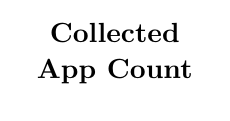
\begin{tikzpicture}
  \node[align=center, text height=3.5ex]{\bfseries Collected\\[1.2pt]\bfseries App Count};
\end{tikzpicture}
 & \bfseries LOC & \bfseries Opriv & \bfseries UPriv &

   % \resizebox {12ex} {5ex} {
        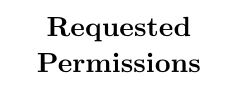
\begin{tikzpicture}
            \node[align=center, text height=3.0ex]{\bfseries Requested\\[1.2pt]\bfseries Permissions};
        \end{tikzpicture}
   % }

 \\ \hline

	%% Not sure if I should show these years
 	%2009 &  4,393  & 1.8 & 1.4 & 2.7  \\ \hline
	%2010 &  9,553  & 2.5 & 1.4 &  3.1  \\ \hline
	2011 & 2,898 &  25,549 & 2.1 & 2.3 & 3.9   \\ \hline
	2012 & 6,020 & 38,183 & 2.3 & 2.4 & 4.8   \\ \hline
	2013 & 17,466 & 83,445  & 2.3 & 2.9 & 5.9   \\ \hline
	2014 & 32,351 & 206,903  & 3.3 & 3.3 & 9.2  \\ \hline
	2015 & 5,382 & 248,802 & 3.6 & 5.3 & 10  \\ \hline

  \end{tabular}
 % } % scalebox
  \end{center}
\end{table}







We next compared how Android malware and Google Play apps are evolving on an annual basis in terms of size (LOC) and requested permissions. We separated the apps collected from the Contagio Mobile Mini Dump into those created in or before 2012, 2013, 2014, and 2015. The results of this analysis are shown in Figure~\ref{fig:Evolution}.



%Figure~\ref{fig:malwareEvolutionLOC} and Figure~\ref{fig:malwareEvolutionPriv}.



%Figure~\ref{fig:Evolution}.

\begin{minipage}{1.0\linewidth}

          \begin{figure}[H]
          \center
              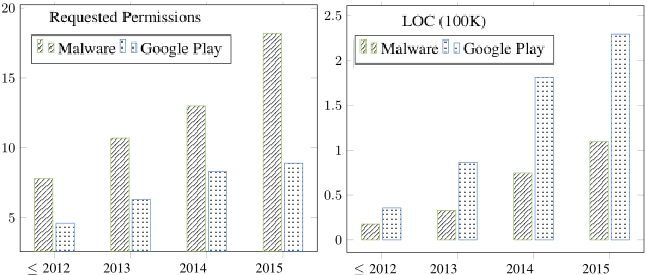
\includegraphics[width=\linewidth]{images/Evolution.png}
              \caption{Evolution of Apps by Permissions \& LOC} % fix image
              \label{fig:Evolution}
          \end{figure}
      \end{minipage}

% Colors used for bar chart
\definecolor{bblue}{HTML}{4F81BD}
\definecolor{ggreen}{HTML}{9BBB59}

%% We did not use apps from the Malware Genome Project since we were unable to collect accurate date information for these apps. -- These were used


% \begin{minipage}{\linewidth}
%      \centering
%      \begin{minipage}{0.45\linewidth}
%          \begin{figure}[H]
%              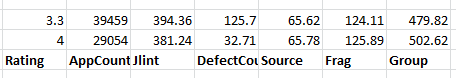
\includegraphics[width=\linewidth]{images/overandunder10Kdownloads_temp.png}
%              \caption{This is the first figure}
%          \end{figure}
%      \end{minipage}
%      \hspace{0.05\linewidth}
%      \begin{minipage}{0.45\linewidth}
%          \begin{figure}[H]
%              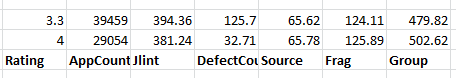
\includegraphics[width=\linewidth]{images/overandunder10Kdownloads_temp.png}
%              \caption{This is the second figure}
%          \end{figure}
%      \end{minipage}
%  \end{minipage}


 %\begin{minipage}{\linewidth}

%%%      \begin{minipage}{0.45\linewidth}
%%%          \begin{figure}[H]
%%%              \begin{tikzpicture}
%%%                    \begin{axis}[
%%%                        ybar,
%%%                    %	scale only axis,
%%%                        enlargelimits=0.15,
%%%                        legend style={at={(0.5,.9)},
%%%                          anchor=north,legend columns=-1},
%%%                          ylabel=LOC (100K),
%%%                    %   ylabel={\#participants},
%%%                        symbolic x coords={$\leq $ 2012,2013,2014,2015},
%%%                        xtick=data,
%%%                    %    nodes near coords,
%%%                    %    nodes near coords align={vertical},
%%%                    	xticklabel style={text width=4em, font=\small},
%%%                    	bar width=12pt
%%%                        ]
%%%
%%%                    %%% For LOC
%%%                    %% Malware
%%%                    \addplot [style={ggreen,pattern=north east lines,mark=none}]coordinates {($\leq $ 2012,17693.375)(2013,32988.662)(2014,7 4606.432)(2015,109947.075) };
%%%
%%%                    %% GP
%%%                    \addplot [style={bblue,pattern=dots,mark=none}]coordinates {($\leq $ 2012,35645)(2013,86482)(2014,181225)(2015,229355) };
%%%
%%%                    \legend{Malware, Google Play}
%%%                    \end{axis}
%%%                    \end{tikzpicture}
%%%                    \caption{Evolution of Apps - LOC}
%%%                    \label{fig:malwareEvolutionLOC}
%%%          \end{figure}
%%%      \end{minipage}
%%%      \hspace{0.05\linewidth}
%%%      \begin{minipage}{0.45\linewidth}
%%%          \begin{figure}[H]
%%%             \begin{tikzpicture}
%%%                \begin{axis}[
%%%                    ybar,
%%%                %	scale only axis,
%%%                    enlargelimits=0.15,
%%%                    legend style={at={(0.5,.9)},
%%%                      anchor=north,legend columns=-1},
%%%                      ylabel=Requested Permissions,
%%%                %   ylabel={\#participants},
%%%                    symbolic x coords={$\leq $ 2012,2013,2014,2015},
%%%                    xtick=data,
%%%                %    nodes near coords,
%%%                %    nodes near coords align={vertical},
%%%                	xticklabel style={text width=4em, font=\small},
%%%                	bar width=12pt
%%%                    ]
%%%
%%%                %%% For Priv
%%%                %% Malware
%%%                \addplot [style={ggreen,pattern=north east lines,mark=none}]coordinates {($\leq $ 2012,7.8)(2013,10.7)(2014,13)(2015,18.2) };
%%%
%%%                %% GP
%%%                \addplot [style={bblue,pattern=dots,mark=none}]coordinates {($\leq $ 2012,4.61)(2013,6.3)(2014,8.3)(2015,8.9) };
%%%
%%%            \legend{Malware, Google Play}
%%%            \end{axis}
%%%            \end{tikzpicture}
%%%            \caption{Evolution of Apps - Permissions}
%%%            \label{fig:malwareEvolutionPriv}
%%%          \end{figure}
%%%      \end{minipage}
%%%  \end{minipage}



%%%% -----------

%%%%% -----------
%%% Colors used for bar chart
%\definecolor{bblue}{HTML}{4F81BD}
%\definecolor{ggreen}{HTML}{9BBB59}
%
%\begin{figure}[]
%\center
%%\vspace{-0.05in}
%\begin{tikzpicture}
%\begin{axis}[
%    ybar,
%%	scale only axis,
%    enlargelimits=0.15,
%    legend style={at={(0.5,.9)},
%      anchor=north,legend columns=-1},
%      ylabel=LOC (100K),
%%   ylabel={\#participants},
%    symbolic x coords={$\leq $ 2012,2013,2014,2015},
%    xtick=data,
%%    nodes near coords,
%%    nodes near coords align={vertical},
%	xticklabel style={text width=4em, font=\small},
%	bar width=12pt
%    ]
%
%%%% For LOC
%%% Malware
%\addplot [style={ggreen,pattern=north east lines,mark=none}]coordinates {($\leq $ 2012,17693.375)(2013,32988.662)(2014,7 4606.432)(2015,109947.075) };
%
%%% GP
%\addplot [style={bblue,pattern=dots,mark=none}]coordinates {($\leq $ 2012,35645)(2013,86482)(2014,181225)(2015,229355) };
%
%
%
%
%\legend{Malware, Google Play}
%\end{axis}
%\end{tikzpicture}
%\caption{Evolution of Apps - LOC}
%\label{fig:malwareEvolutionLOC}
%\end{figure}
%
%
%%%% analyze the results
%
%\begin{figure}[]
%\center
%%\vspace{-0.05in}
%\begin{tikzpicture}
%\begin{axis}[
%    ybar,
%%	scale only axis,
%    enlargelimits=0.15,
%    legend style={at={(0.5,.9)},
%      anchor=north,legend columns=-1},
%      ylabel=Requested Permissions,
%%   ylabel={\#participants},
%    symbolic x coords={$\leq $ 2012,2013,2014,2015},
%    xtick=data,
%%    nodes near coords,
%%    nodes near coords align={vertical},
%	xticklabel style={text width=4em, font=\small},
%	bar width=12pt
%    ]
%
%
%
%%%% For Priv
%%% Malware
%\addplot [style={ggreen,pattern=north east lines,mark=none}]coordinates {($\leq $ 2012,7.8)(2013,10.7)(2014,13)(2015,18.2) };
%
%%% GP
%\addplot [style={bblue,pattern=dots,mark=none}]coordinates {($\leq $ 2012,4.61)(2013,6.3)(2014,8.3)(2015,8.9) };
%
%
%
%
%\legend{Malware, Google Play}
%\end{axis}
%\end{tikzpicture}
%\caption{Evolution of Apps - Permissions}
%\label{fig:malwareEvolutionPriv}
%\end{figure}


\noindent
\textbf{Analysis:} We found that malicious apps are growing on an annual basis in both LOC and requested permissions. An interesting discovery is that although both are consistently growing, Google Play apps are larger in terms of LOC, but are smaller in the number of requested permissions. Our findings have several important implications for both general app development, and malware research. For developers of benign apps, indications are that apps will continue to grow in terms of LOC and in requested permissions. This is significant for several reasons. The first is that with more permissions, developers will need to be better educated about the permissions they use and diligent to ensure that they are properly using them. This will be further complicated by Google's move to a new permission structure in Android 6.0 which will allow apps to request permissions at runtime instead of only upon installation of the app.

Benign Apps are becoming larger in terms of LOC, which likely means that teamwork will be increasingly more important since more developers will be needed to create an maintain the apps. With more developers being involved in the app, fundamental software engineering skills such as communication, documentation, diverse team roles, testing and adhering to coding standards will become increasingly important~\cite{Pressman:2009:SEP:1593949}. On average, malware is smaller in terms of LOC in comparison to benign apps, but is growing and requesting more permissions on an annual basis. There are a variety of current malware detection techniques including API tracing~\cite{6298136}, behavioral based techniques~\cite{burguera2011crowdroid, shabtai2012andromaly}, permission based systems~\cite{talha2015apk}, and signature based approaches~\cite{Feng:2014:ASD:2635868.2635869}. Larger software will make many of these processes more difficult and time consuming, leading for the need for different and more efficient processes.

\begin{table}[ht]
\begin{center}
\caption{Malware Permission Growth By Year}
\label{Table:malPrivGrowth}
 \begin{tabular}{ | l | c | c | c | c |} \hline

& \multicolumn{4}{ c | }{\bfseries \% Occuring} \\ \hline
	  \bfseries Permission & \bfseries   2012 & \bfseries 2013  & \bfseries 2014 & \bfseries 2015 \\ \hline %\hline

	RECEIVE\_BOOT\_COMPLETED & 55 & 52 & 71& 86 \\ \hline
	READ\_CONTACTS & 36 & 55&  41& 68 \\ \hline
	SYSTEM\_ALERT\_WINDOW &1 & 16 &  27 & 61 \\ \hline
	WAKE\_LOCK &34 & 19 & 41 &54 \\ \hline
	GET\_TASKS &17 & 25 & 43 & 39 \\ \hline	
	%MOUNT\_UNMOUNT\_FILESYSTEMS & 10 & 19 & 14 & 32 \\ \hline

  \end{tabular}
\end{center}
\end{table}


We next chose to examine the usage rate in several of the permission requests which were growing at the most substantial rate between 2012 and 2015 in malware. The results of this are shown in Table~\ref{Table:malPrivGrowth}. These results indicate that malware is using these permissions much more frequently now, than even a few years ago. For instance, the usage of \texttt{SYSTEM\_ALERT\_WINDOW} has gone from appearing in 1\% of malware in 2012, to 61\% in 2015. This permission allows an an app to create new windows on the Android UI, and may often be used by malware to display a message in an attempt to convey misinformation to the user. Security researchers can analyze these trends to see how malware is evolving over time and the different types of attacks they are attempting to perform using these extra permissions. This information could prove to be invaluable for both detecting and countering the negative effects of malware.

%The new Android 6.0 permissions model substantially changed both how app permissions are requested, along with how many permissions are categorized (normal or dangerous). For example, the \texttt{INTERNET} permission previously required a user's authorization for an app's use, however in Android 6.0 it is defined as a 'Normal' permission, meaning it does not require a user's authorization. Understanding the permission trends in malware is paramount for understanding any further adjustments which are required to any updated permissions model. Possible alterations could include the further consolidations for permissions and their groups, adjustment of `Normal' and `Dangerous'  permission groups, or even the creation of new permissions.

%Although there should be further analysis of Android 6.0 malware before any definitive recommendations are made, it is concerning that three of the top 10 most requested malware permissions of 2015 (\texttt{INTERNET}, \texttt{ACCESS\_NETWORK\_STATE} and \\ \texttt{ACCESS\_WIFI\_STATE}) are considered to be `Normal' permissions in Android 6.0, meaning the user will not be prompted to give the app access to these permissions.



\section{Public Dataset \& Website}
\label{sec:dataset}

\textbf{Dataset}: Our dataset is available from our publicly accessible GitHub repo\footnote{\ifisnopii https://github.com/DroidDarwin \else https://github.com/-Hidden- \fi}, which includes the scripts used for collecting apps and invoking the static analysis tools. The SQLite database with our complete results is updated on a regular basis from our collection and analysis software. The goal of this dataset is to allow future researchers to both learn from and expand upon our work. This dataset contains the information collected from Google Play, and the results of our static analysis tools. The raw data used in our analysis is available in three SQLite databases from our public GitHub repository, with one each for the malware data from Contagio and the Malware Genome projects, and a third for the collected information from Google Play. Unfortunately, the actual malicious APK files may only be obtained from the Contagio and Genome websites due to usage agreements.

%\subsection{Website}
\noindent
\textbf{Website}: Our project website (\textbf{\ifisnopii http://darwin.rit.edu \else http://hiddenToKeepAnonymous\fi}) contains information about our project, links to our GitHub repository, and a robust reporting tool which will allow users to create their own datasets from over 70,000 analyzed applications. New apps will be added on a regular basis as they are collected and analyzed from Google Play.


\section{Limitations \& Future Work}
\label{sec:limitations}


While static analysis tools have demonstrated their value in numerous previous works~\cite{Felt:2011:APD:2046707.2046779, Pearce:2012:APS:2414456.2414498}, it is unreasonable to expect that any tool will ever be flawless and that no static analysis tool is perfect and generally inherently contains limitations~\cite{chess2004static}. Although Stowaway is a powerful static analysis tool which has been used in previous research~\cite{Felt:2011:APD:2046707.2046779, Pearce:2012:APS:2414456.2414498}, it does suffer from drawbacks. Stowaway's own authors state that the tool only achieves 85\% code coverage~\cite{Felt:2011:APD:2046707.2046779}, so the under \& over-permissions reported by this tool are imperfect. Additionally, any reported vulnerabilities or defects by a static analysis tool should be deemed as~\emph{possible} vulnerabilities or defects, not necessarily actual ones. There is also the possibility of issues in the reverse engineering process of the apps, but we are confident in the process due to its demonstrated effectiveness and accuracy in existing research~\cite{krutz2015FDroid, Lee_2013}, and due to our manual verification of some of the apps.


%%% Maybe add back in?
%Identifying possible vulnerabilities or security risks is extremely difficult, and like any static analysis tool Androrisk is only capable of making educated observations about the risk level of an app and that more substantial risk assessments will require a far more substantial level of analysis, which will likely include a manual investigation of the app. Due to the large number of examined apps in our study, this thorough level of analysis was not practical. Even with almost certain imperfections, we believe that Androrisk was a good choice due to its ability to quickly analyze apps and its use in existing research~\cite{krutz2015FDroid}.

%We compiled much of our data through reverse engineering APK files from the Google Play store. While similar reverse engineering techniques have been successfully used in previous works~\cite{Lee_2013,6687155}, no reverse engineering process can ever be expected to be totally accurate. However, based on manually verifying a small subset of our results and previous research, we have a high confidence in our reverse engineering process.


We only analyzed apps from Google Play and not other sources such as the Amazon Appstore\footnote{\url{http://www.amazon.com/mobile-apps/b?node=2350149011}} or F-Droid, which would have led to more varied application origins. However, we feel the diversity of our apps was already quite robust since we collected 70,785  applications from 41 categories. We also only examined free applications in our research due to cost constrains. Thus, the measurements comparison of apps is not representative of the entire Google Play market. Our results only apply as an evaluation of free apps, not paid apps.

We analyzed 1,420 malicious Android apps in a variety of areas. Although this represents a substantial number of malicious apps, it obviously represents only a minor portion of all Android malware. Attaining Android malware samples is a difficult task since they are often difficult to identify, and are often not widely publicized or shared for a variety of reasons, including the fear that this may only lead to them spreading.


%%  We only analyzed free apps, and an interesting study would be to compare the free and paid apps using a similar process as ours.

While we have demonstrated profound results through the collection of over 70,000 Android apps, future work may be conducted in several key areas. An interesting topic would be to analyze how apps evolve over time through the examination of numerous released versions of the same app, and not through the aggregate values of apps as we have done. Android 6.0 received a massive permissions overhaul and work may be done to see how this new release affects how developers use permissions. Naturally more apps can always be examined, and with new apps being released on a daily basis the process is never ending.

%We used Stowaway to discover over-permissions in apps. While permission misuse is a possible vulnerability, over-permissions do not necessarily mean permission leaking, which is when an unprivileged app has access to permissions which is was never granted. Often, an app is allowed access to permissions by inheriting permissions from another app with the same signing key~\cite{felt2011permission, grace2012systematic}. Future work using permission leak detection tools such as IntentFuzzer~\cite{Yang:2014:IDC:2590296.2590316} can be done to include this metric in the app's security analysis.





%   ? Adoption rates of new Android APis    - Might not be a great idea to include this
%   Further undestanding of what these values mean
%   Website enhancements


%%  What was said in evaluations that we can address here



\section{Conclusion}
\label{sec: conclusion}

%% Probably clean this up a bit
In this paper, we described our collection and analysis process used to examine over 70,000 malicious and benign Android apps from several security and quality perspectives. Some of the primary discoveries include significant differences in permissions usage across app categories and malware, a comparison of the top over-permissions in benign and malicious apps, the discovery of only a weak correlation between an app's quality and security, a comparison benign and malicious apps in terms of several security based metrics, and that both benign and malicious apps are growing on an annual basis. Our work has laid the foundation for important future research in analyzing both quality and security issues in Android apps, along with providing an invaluable dataset for other researchers to use in their own studies.



%%% Remove this section if there are space issues
\section*{Acknowledgements}

This work is partially funded by a development grant from the Rochester Institute of Technology.



%\balance % Not needed for llncs
\bibliographystyle{abbrv}
\bibliography{SecurityDarwin}


\


\end{document}



%% Todo
% Clean up all format
% Fix checkmark
% Make images smaller
% Remove some bib items? (there are some duplicates)
